\chapter{Analisi sperimentale: NTPsec}
\label{cha:NTPsec} \label{cha:NTPsec}

Il presente capitolo è dedicato all’analisi dei dati raccolti per il demone
\textbf{NTPsec}, con l’obiettivo di valutarne il comportamento al variare delle
condizioni di rete introdotte nei tre scenari sperimentali. L’attenzione è rivolta
all’esame delle principali metriche di sincronizzazione temporale osservate durante
la fase di testing, al fine di evidenziare l’eventuale impatto del progressivo
incremento degli impairment di rete sulla stabilità del sistema e sulla qualità
del processo di sincronizzazione.

L’analisi è organizzata per metrica. Per ciascuna grandezza considerata viene condotto
un confronto sistematico tra i tre scenari sperimentali definiti in precedenza,
corrispondenti a differenti livelli di degrado della rete (\textit{low}, \textit{medium},
\textit{high}). Tale confronto si basa sull’osservazione dei dati raccolti e
sulla loro rappresentazione grafica, con lo scopo di mettere in evidenza eventuali
variazioni nel comportamento del demone in termini di accuratezza della sincronizzazione,
variabilità delle misurazioni e dinamica di convergenza.

\vspace{0,2 cm}
\begin{table}[h]
  \centering
  \caption{Scenario matrix used in Phase 3 (T2 with NETEM)}
  \begin{tabular}{|c|c|c|c|c|c|}
    \hline
    \textbf{Scenario} & \textbf{Delay} & \textbf{Jitter} & \textbf{Loss} & \textbf{Reorder} & \textbf{Rate Limit} \\
    \hline
    LOW               & 5 ms           & 1 ms            & 0.1\%         & 1\%              & 50 Mbit             \\
    \hline
    MEDIUM            & 15 ms          & 5 ms            & 0.5\%         & 5\%              & 20 Mbit             \\
    \hline
    HIGH              & 60 ms          & 20 ms           & 10\%          & 20\%             & 5 Mbit              \\
    \hline
  \end{tabular}
  \label{tab:scenario_matrix}
\end{table}
\vspace{0,4 cm}

Nel caso di \textbf{NTPsec}, l’analisi si concentra su tre metriche principali:
\textbf{delay}, \textbf{jitter} e \textbf{offset}. Tali grandezze consentono di caratterizzare,
rispettivamente, il tempo di propagazione dei pacchetti NTP, la variabilità
temporale delle misurazioni e lo scostamento tra il clock locale e il clock di
riferimento. La loro evoluzione nei diversi scenari permette quindi di valutare la
robustezza del demone rispetto al degrado delle condizioni di rete e di analizzare
la qualità del processo di sincronizzazione in termini sia di stabilità sia di accuratezza.

I dati oggetto dell’analisi sono stati raccolti secondo la metodologia sperimentale
illustrata nei capitoli precedenti. In questa sede, pertanto, non vengono
ripresi gli aspetti relativi alla configurazione dell’ambiente di prova o alla
disposizione della topologia, ma si assume come riferimento l’insieme delle misurazioni
già ottenute per ciascuna metrica e per ciascuno scenario di rete. Nel caso
specifico di \textbf{NTPsec}, le misurazioni considerate sono state rilevate sui
nodi \textit{client} e \textit{boundary} della topologia, in coerenza con il ruolo
da essi ricoperto nel processo di sincronizzazione.

Ciascuna sezione seguente è quindi dedicata a una singola metrica e presenta,
per i tre scenari sperimentali, i risultati osservati e il relativo confronto interpretativo,
con l’obiettivo di individuare eventuali differenze significative tra le
condizioni di rete considerate e valutarne gli effetti sul comportamento del
demone.

\newpage
\section{Analisi dati: "Delay"}
\begin{figure}[h]
  \centering

  \begin{subfigure}
    {0.32\textwidth}
    \centering
    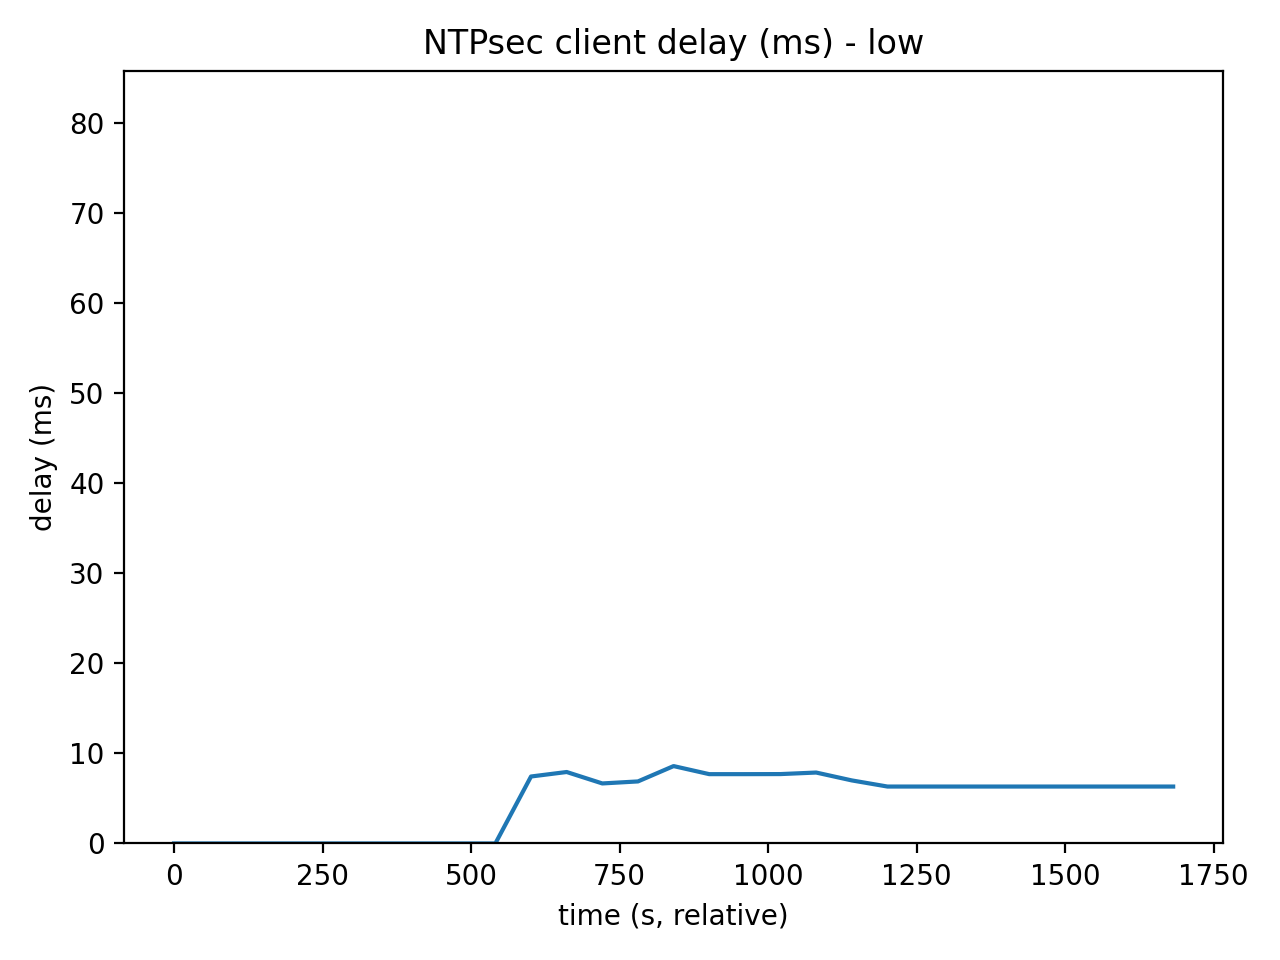
\includegraphics[width=\linewidth]{
      images/data_plots/plots_ntpsec/ntpsec_client_low_delay_ms.png
    }
    \caption{Scenario LOW}
  \end{subfigure}
  \hfill
  \begin{subfigure}
    {0.32\textwidth}
    \centering
    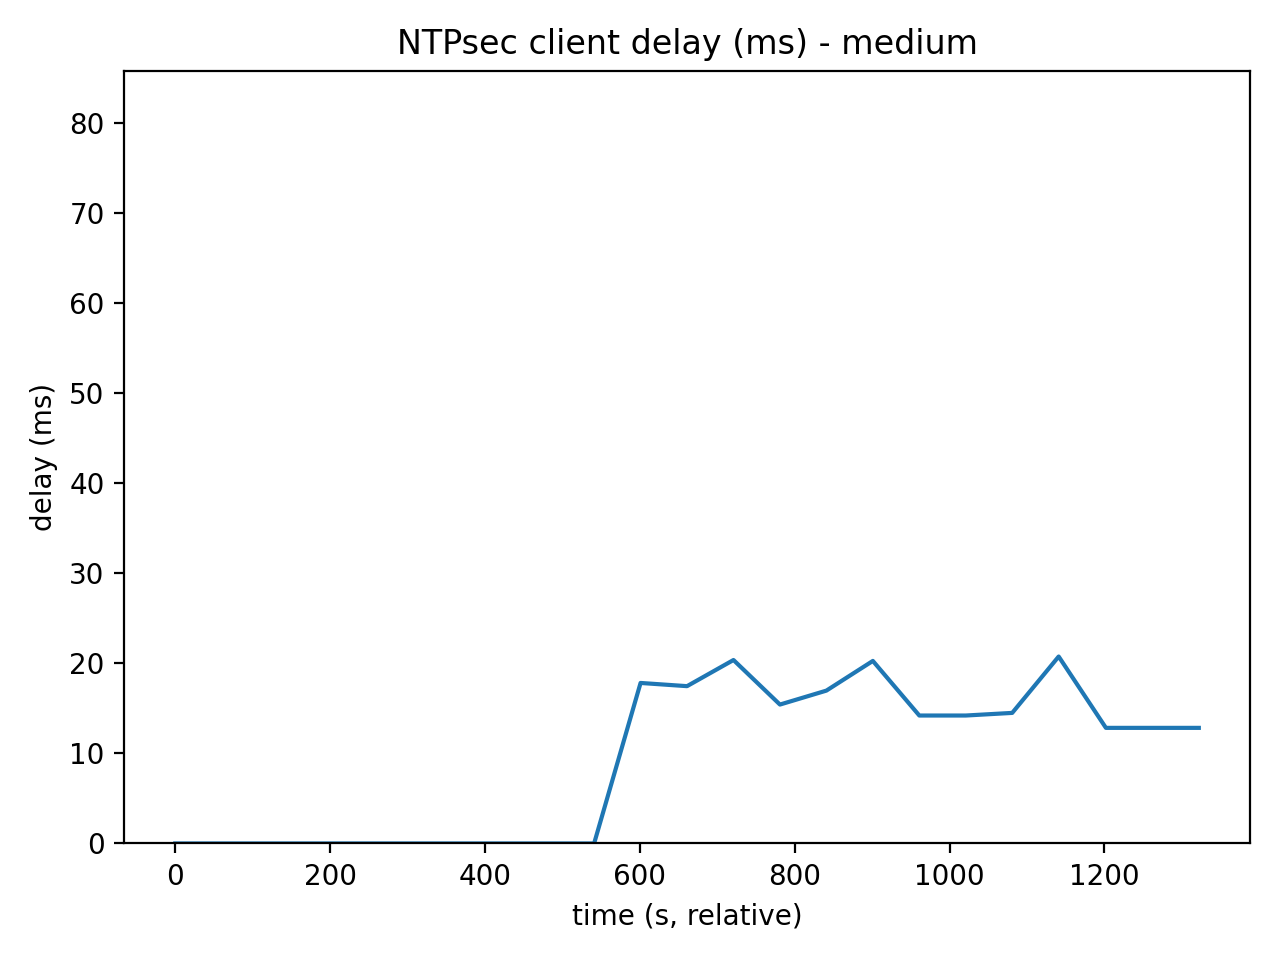
\includegraphics[width=\linewidth]{
      images/data_plots/plots_ntpsec/ntpsec_client_medium_delay_ms.png
    }
    \caption{Scenario MEDIUM}
  \end{subfigure}
  \hfill
  \begin{subfigure}
    {0.32\textwidth}
    \centering
    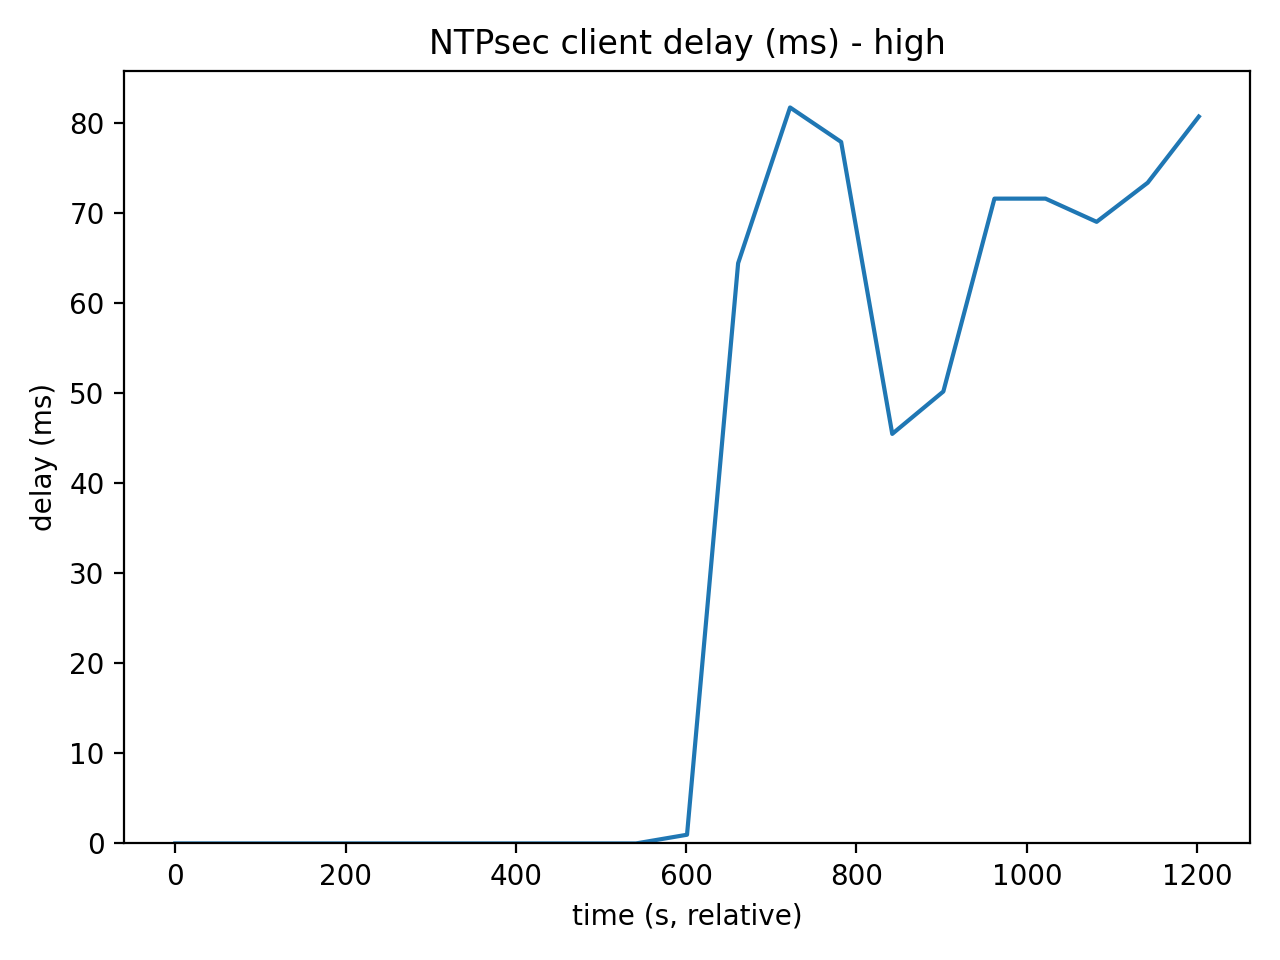
\includegraphics[width=\linewidth]{
      images/data_plots/plots_ntpsec/ntpsec_client_high_delay_ms.png
    }
    \caption{Scenario HIGH}
  \end{subfigure}

  \caption{Comparazione della performance - nodo: \textit{clientntp}}
  \label{fig:scenario_comparison}
\end{figure}

L’analisi del \textbf{delay} misurato sul nodo \textit{clientntp} per il demone \textbf{NTPsec}
evidenzia una dipendenza marcata dal livello di impairment introdotto nei tre
scenari sperimentali. In tutti i casi, la porzione iniziale della serie è
caratterizzata da uno stato di inizializzazione, identificato da \texttt{refid=.INIT.},
\texttt{stratum=16}, \texttt{selected=False} e \texttt{reach=0}. Tale intervallo
non rappresenta il regime operativo della sincronizzazione e non viene quindi
considerato nel confronto tra scenari, che viene invece condotto a partire dal primo
campione valido, corrispondente in tutti i casi a circa 601 secondi di tempo
relativo.

Nello scenario \textit{low}, il delay assume valori contenuti e presenta un
andamento fortemente regolare. Sui campioni validi si osserva un valore medio pari
a 6.96 ms, con deviazione standard di 0.75 ms, minimo di 6.32 ms e massimo di 8.59
ms. Il range complessivo risulta quindi pari a 2.27 ms. La serie mostra oscillazioni
modeste e una progressiva stabilizzazione su valori prossimi a 6.3 ms, indicando
che, in presenza di impairment ridotti, il percorso di rete mantiene
caratteristiche sufficientemente stabili da non introdurre ritardi significativi
né elevata variabilità nelle misure.

Nel caso \textit{medium}, il delay cresce in modo netto e si colloca su una
fascia di valori sensibilmente superiore. La media dei campioni validi è pari a 16.18
ms, con deviazione standard di 2.96 ms, minimo di 12.83 ms e massimo di 20.75 ms.
Rispetto allo scenario \textit{low}, il delay medio risulta quindi più che
raddoppiato, mentre aumentano in modo evidente anche la dispersione e l’ampiezza delle
oscillazioni. L’andamento della serie resta leggibile e non mostra fenomeni di
divergenza, ma la misura risulta meno regolare e più sensibile alla variabilità introdotta
dalla rete.

Lo scenario \textit{high} presenta il comportamento più degradato. Al netto del primo
campione selezionato, che assume carattere transitorio rispetto al resto della
serie, il delay si colloca stabilmente in una fascia elevata, con media pari a
68.57 ms, deviazione standard di 12.18 ms, minimo di 45.46 ms e massimo di 81.69
ms. Il confronto con gli altri scenari evidenzia un incremento molto marcato: il
delay medio risulta circa 4.2 volte superiore rispetto al caso \textit{medium} e circa
9.8 volte superiore rispetto al caso \textit{low}. In questo scenario, oltre al
forte aumento del livello medio, si osserva anche una variabilità significativamente
maggiore, indice di una condizione di rete fortemente instabile dal punto di
vista temporale.

Nel complesso, il confronto tra i tre scenari mostra una progressione monotona del
delay al crescere della severità degli impairment di rete. Il passaggio da
\textit{low} a \textit{medium} comporta un incremento sensibile ma ancora
compatibile con un regime relativamente stabile; il passaggio da \textit{medium}
a \textit{high} introduce invece un cambiamento di regime molto più marcato, in
cui il ritardo osservato dal client cresce drasticamente e la misura perde gran
parte della propria regolarità. La metrica del delay risulta pertanto particolarmente
efficace nel mettere in evidenza l’impatto del degrado della rete sul comportamento
del client NTPsec.